\documentclass{article}
\usepackage[utf8]{inputenc}
\usepackage[T1]{fontenc}
\usepackage[slovak]{babel}
\usepackage{geometry}
\geometry{a4paper, margin=1in}
\usepackage{hyperref}
\usepackage{graphicx}

\title{\Huge Používateľská príručka k aplikácii Šípka}
\author{Mgr. Lukáš Gajdošech}
\date{\today}

\begin{document}

\maketitle

\section*{Úvod}
Aplikácia Šípka je interaktívna webová aplikácia určená na riešenie a tvorbu labyrintov pomocou umiestňovania šípok. 
Umožňuje študentom riešiť labyrinty v režime študenta a učiteľom vytvárať a upravovať labyrinty v režime učiteľa. 
Aplikácia podporuje načítanie a ukladanie máp, vizualizáciu riešení, automatické generovanie a riešenie labyrintov.

\section*{Režim študenta (main.html)}

\begin{center}
    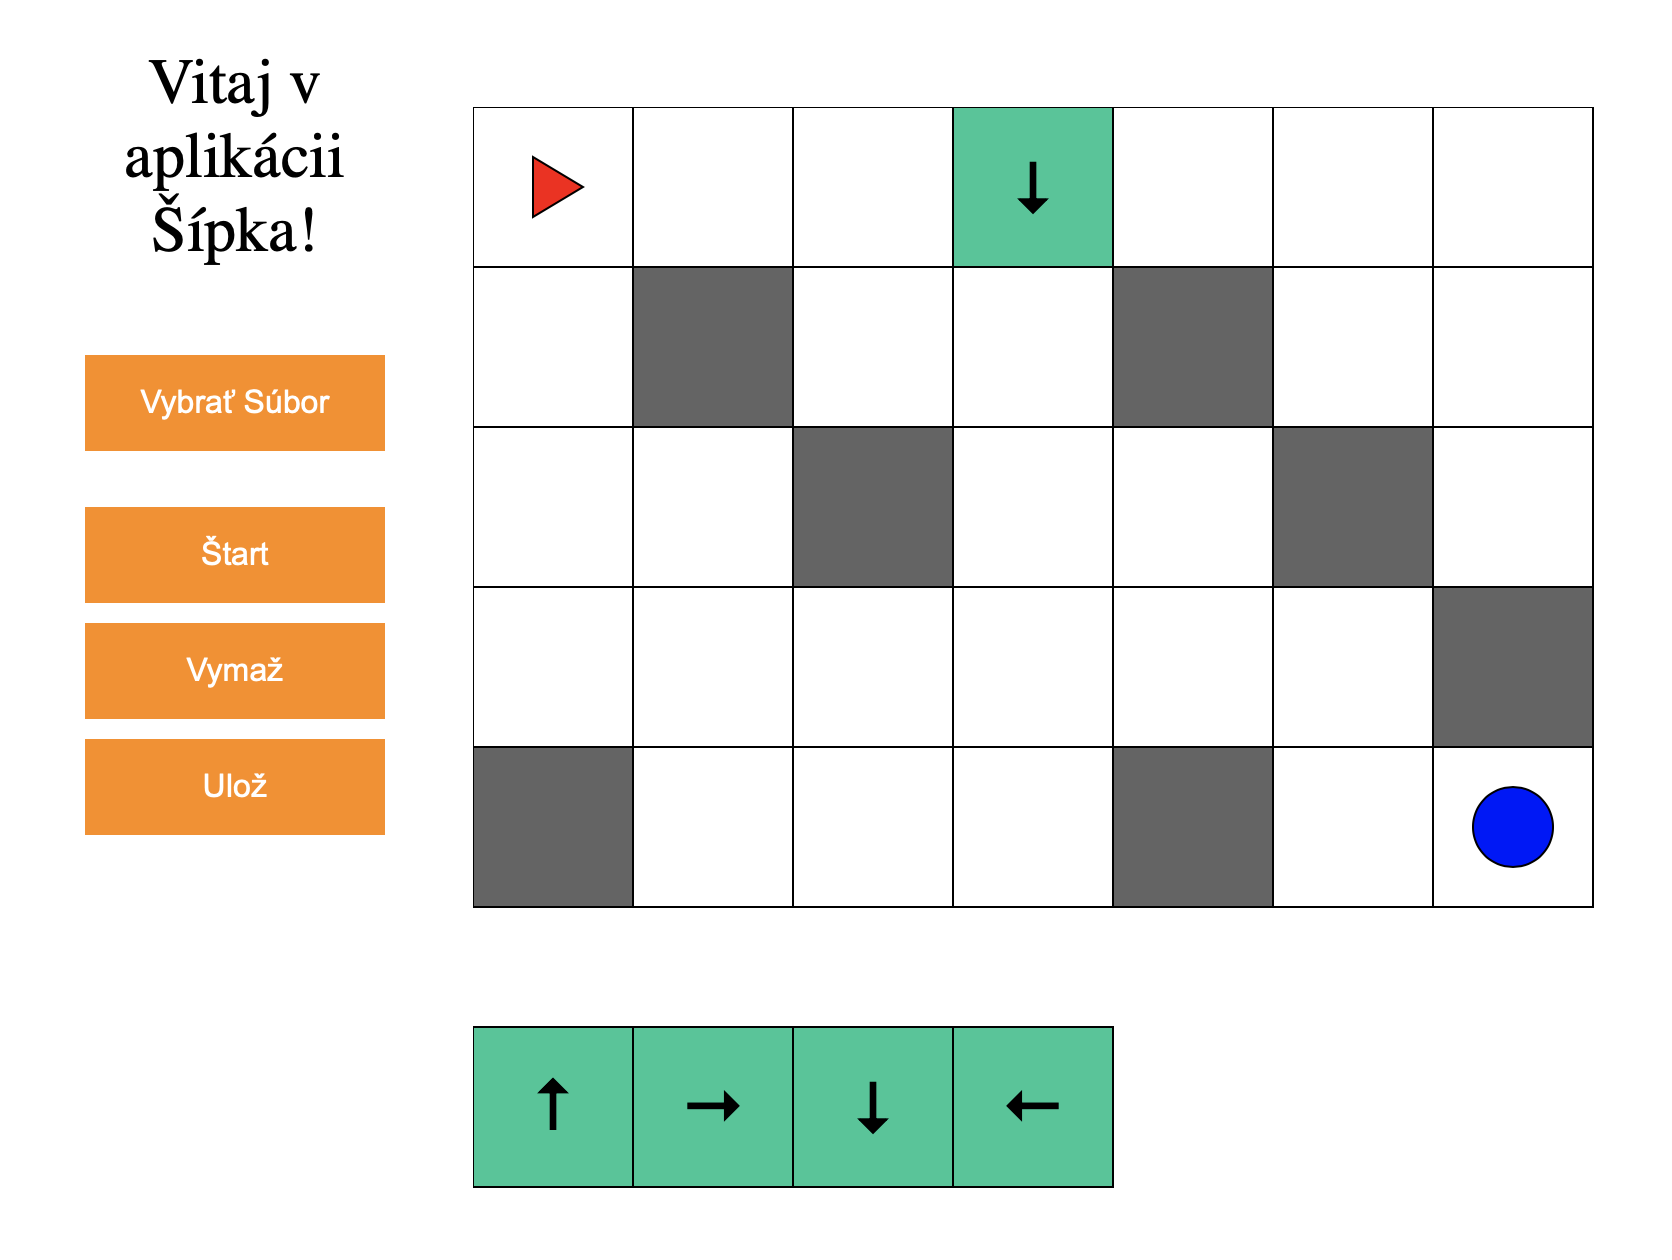
\includegraphics[width=12cm]{student.png}
\end{center}

V režime študenta môžu používatelia interaktívne umiestňovať šípky na hraciu plochu a tým usmerňovať pohyb robota cez labyrint.
Robot reprezentovaný červeným trojuholníkom sa samostatne vždy hýbe smerom vpred, pričom pri náraze na prekážku sa otáča vpravo. 
Cieľom hráča je umiestniť najmenší potrebný počet šípok na dosiahnutie cieľa znázorneného modrým kruhom.

\newpage

\subsection*{Tlačidlá a ich funkcie}
\begin{itemize}
    \item \textbf{Vybrať Súbor}: Načítanie labyrintu z lokálneho súboru, spustí dialógové okno pre výber súboru.
    \item \textbf{Štart/Pauza/Pokračuj}: Slúži na spustenie, pozastavenie alebo pokračovanie pohybu robota. 
    Text na tlačidle sa teda dynamicky mení podľa aktuálneho stavu.
    \item \textbf{Vymaž}: Resetuje aktuálny stav labyrintu a vymaže všetky umiestnené šípky.
    \item \textbf{Ulož}: Umožňuje uložiť aktuálny stav labyrintu aj so šípkami do súboru.
    \item \textbf{Riešenie}: Zobrazuje optimálne riešenie labyrintu, ak existuje. 
    Toto tlačidlo sa zobrazí, až po 2 neúspešných riešeniach labyrintu, tj. takých, ktoré obsahovali viac šípok ako je potrebné.
\end{itemize}

\subsection*{Interaktívny panel so šípkami}
\begin{itemize}
    \item \textbf{Umiestnenie šípok}: Šípky zo spodnej lišty sa môžu ťahať myšou na hraciu plochu, kde určujú smer pohybu robota.
    \item \textbf{Premiestnenie šípok}: Umiestnené šípky môžu byť dodatočne premiestnené rovnakým spôsobom. 
    Prípadne sa dajú vymazať potiahnutím mimo mapy. 
\end{itemize}

\section*{Režim učiteľa (teacher.html)}

\begin{center}
    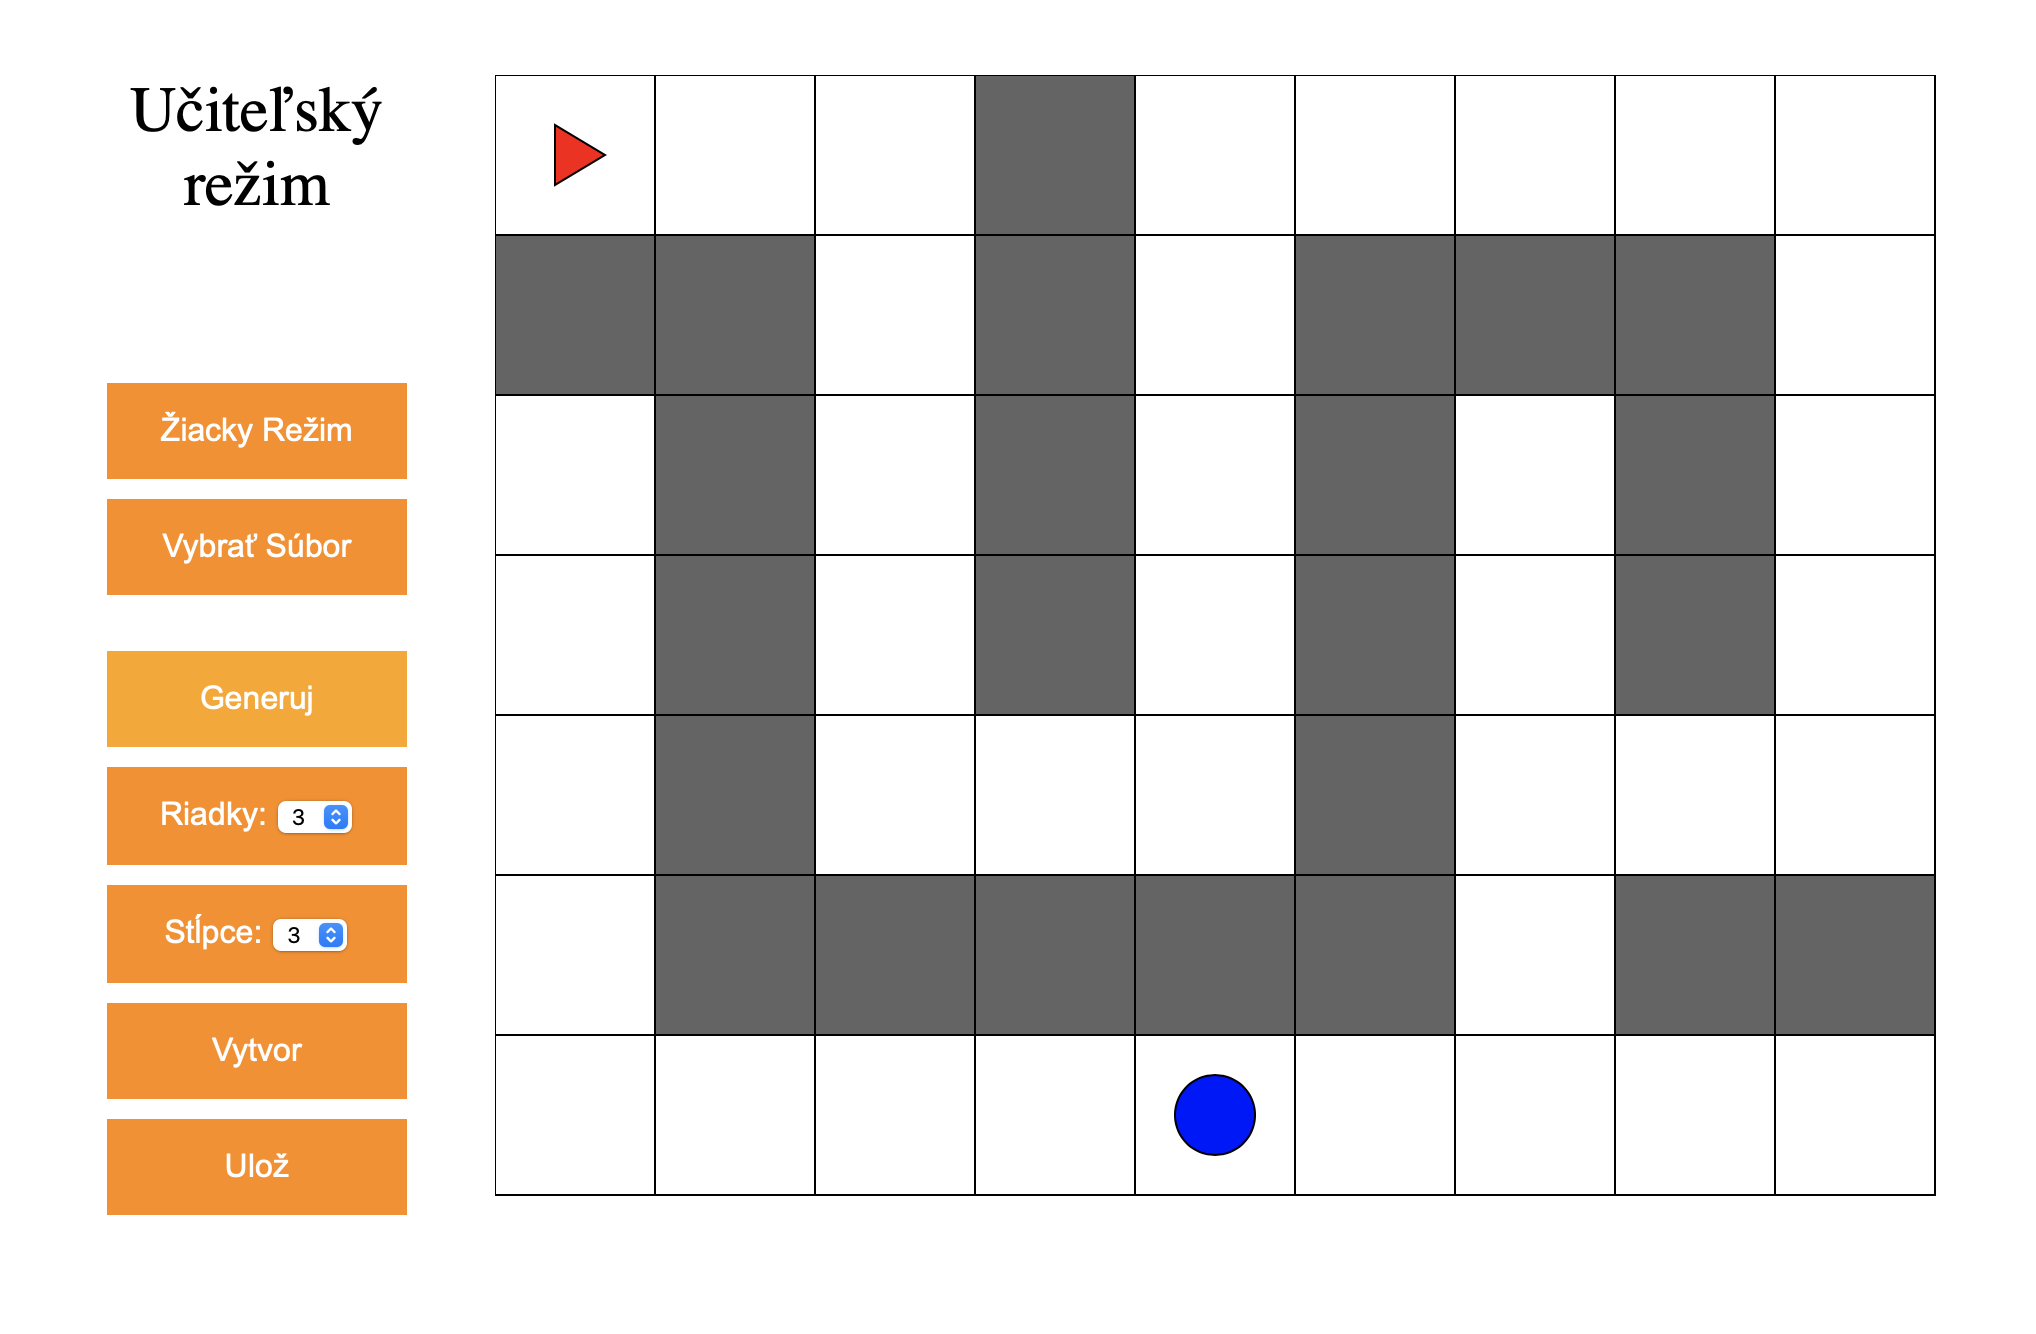
\includegraphics[width=12cm]{teacher.png}
\end{center}

Režim učiteľa poskytuje rozšírené možnosti na tvorbu a úpravu labyrintov, vrátane manuálnej tvorby a automatického generovania.

\subsection*{Tlačidlá a ich funkcie}
\begin{itemize}
    \item \textbf{Žiacky Režim}: Prepne aplikáciu do interaktívneho žiackeho režimu s persistentným zachovaním aktuálnej mapy.
    \item \textbf{Generuj}: Automaticky vygeneruje nový labyrint použitím upraveného Recursive Backtracker\footnote{https://weblog.jamisbuck.org/2011/2/7/maze-generation-algorithm-recap} algoritmu. 
    Náhodne sú určené aj rozmery labyrintu, špecifikácia funguje pre nasledujúce tlačidlo.
    \item \textbf{Vytvor}: Vytvorí prázdny labyrint bez stien s rozmermi zadanými v kolónkach Riadky a Stĺpce. 
    \item \textbf{Ulož}: Umožňuje uložiť vytvorený alebo upravený labyrint do súboru.
\end{itemize}

\subsection*{Interakcia s aplikáciou}
\begin{itemize}
    \item \textbf{Editácia mapy}: Učiteľ môže pridávať alebo odoberať steny v labyrinte kliknutím na príslušné bunky na hracej ploche.
    \item \textbf{Úprava cieľa}: Pozícia cieľa sa dá zmeniť ťahaním myšou. Štart robota je fixne vždy v ľavom hornom rohu.
\end{itemize}

\section*{Scenáre použitia}
\begin{itemize}
    \item \textbf{Vzdelávacie účely}: Učitelia môžu vytvárať labyrinty na testovanie logického myslenia študentov.
    \item \textbf{Súťaže}: Študenti môžu súťažiť v rýchlosti riešenia labyrintov.
    \item \textbf{Sebahodnotenie}: Študenti môžu používať aplikáciu na testovanie a zlepšovanie schopnosti riešiť problémy.
\end{itemize}

\section*{Nastavenie automatického riešenia}

Automatické hľadanie riešenia funguje v samostatnom vlákne, vďaka čomu ostáva hlavné vlákno aplikácie stále interaktívne. 
Algoritmus postupne prehľadáva možné umiestnenia šípok, počnúc riešeniami s jednou šípkou, následne s dvoma, troma, atď. 
Vďaka tomu je zaručené, že vždy ako prvé nájde riešenie s najmenším možným počtom šípok. Jeho správanie možno upraviť zmenou
konštánt v súbore main.html na riadkoch 72-74.

\subsection*{Význam koštánt}
\begin{itemize}
    \item \textbf{EARLY\_STOP} (východzia hodnota: false): Určuje, či má algoritmus vrátiť prvé nájdené riešenie, 
    alebo má prehľadať aj ostatné riešenia s rovnakým počtom šípok a následne vrátiť také, ktoré vyžaduje najmenej krokov robota. 
    Takéto riešenie je zároveň pre študenta často najintuitívnejšie na pochopenie. 
    \item \textbf{MAX\_STEPS} (východzia hodnota: 30): Maximálny povolený počet krokov robota. 
    Riešenia, ktoré by vyžadovali väčší počet krokov algoritmus automaticky zamieta.
    \item \textbf{MAX\_ARROWS} (východzia hodnota: 4): Maximálny povolený počet umiestnených šípok. 
    Ak aktuálny labyrint vyžaduje viac šípok na vyriešenie,
    v programe sa po vyžiadaní riešenia zobrazí hláška, že automatické hľadanie nebolo schopné nájsť riešenie. 
\end{itemize}

Táto príručka poskytuje základné informácie o používaní aplikácie Šípka. Pre ďalšie detaily alebo pomoc sledujte repozitár aplikácie \url{https://github.com/gajdosech2/EduSoft} alebo priamo kontaktujte autora 
\href{mailto:l.gajdosech@gmail.com}{l.gajdosech@gmail.com} 
Pre úplnú technickú špecifikáciu aplikácie si prosím prečítajte \href{https://docs.google.com/document/d/1iO6MmWv0fqi1tS6VNDiRenPgHrlYh8M751RDV6SoXGI/edit?usp=sharing}{Dokument Technickej Špecifikácie}.


\end{document}
